% Graphic for TeX using PGF
% Title: /home/araujo/Dropbox/VerbTeX/LivroComputadores/Pictures/memoria.dia
% Creator: Dia v0.97.3
% CreationDate: Sun May 21 11:59:17 2017
% For: araujo
% \usepackage{tikz}
% The following commands are not supported in PSTricks at present
% We define them conditionally, so when they are implemented,
% this pgf file will use them.
\ifx\du\undefined
  \newlength{\du}
\fi
\setlength{\du}{15\unitlength}
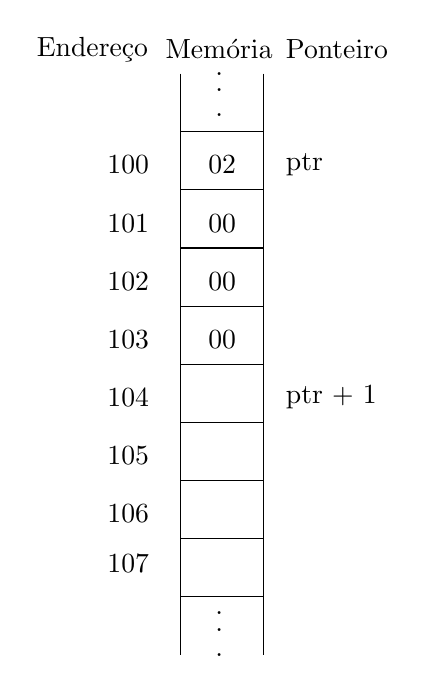
\begin{tikzpicture}
\pgftransformxscale{1.000000}
\pgftransformyscale{-1.000000}
\definecolor{dialinecolor}{rgb}{0.000000, 0.000000, 0.000000}
\pgfsetstrokecolor{dialinecolor}
\definecolor{dialinecolor}{rgb}{1.000000, 1.000000, 1.000000}
\pgfsetfillcolor{dialinecolor}

\draw (27\du,9.4\du)--(27\du,8\du)--(25\du,8\du)--(25\du,9.4\du);
\node at (26\du,8.8\du){02};
\draw (27\du,10.8\du)--(27.\du,9.4\du)--(25\du,9.4\du)--(25\du,10.8\du);
\node at (26\du,10.2\du){00};
\draw (27\du,12.2\du)--(27.\du,10.8\du)--(25\du,10.8\du)--(25\du,12.2\du);
\node at (26\du,11.6\du){00};
\draw (27\du,13.6\du)--(27.\du,12.2\du)--(25\du,12.2\du)--(25\du,13.6\du);
\node at (26\du,13\du){00};
\draw (27\du,15\du)--(27.\du,13.6\du)--(25\du,13.6\du)--(25\du,15\du);

\draw (27\du,16.4\du)--(27.\du,15\du)--(25\du,15\du)--(25\du,16.4\du);

\draw (27\du,17.8\du)--(27.\du,16.4\du)--(25\du,16.4\du)--(25\du,17.8\du);

\draw (27\du,17.8\du)--(27.\du,16.4\du)--(25\du,16.4\du)--(25\du,17.8\du);
%\node at (27.5\du,18.6\du){0110 1100};
\draw (27\du,19.2\du)--(27.\du,17.8\du)--(25\du,17.8\du)--(25\du,19.2\du)--cycle;
\node[anchor=west] at (25.6\du,20.6\du){.};
\node[anchor=west] at (25.6\du,20\du){.};
\node[anchor=west] at (25.6\du,19.6\du){.};

\definecolor{dialinecolor}{rgb}{0.000000, 0.000000, 0.000000}
\pgfsetstrokecolor{dialinecolor}
\draw (25\du,19.2\du)--(25\du,20.6\du);
\draw (27\du,19.2\du)--(27\du,20.6\du);
\draw (25\du,6.6\du)--(25\du,8\du);
\draw (27\du,6.6\du)--(27\du,8\du);
\node[anchor=west] at (25.6\du,7.600000\du){.};
\node[anchor=west] at (25.6\du,7.000000\du){.};
\node[anchor=west] at (25.6\du,6.600000\du){.};
\node[anchor=west] at (23\du,8.8\du){100};
\node[anchor=west] at (23\du,10.2\du){101};
\node[anchor=west] at (23\du,11.6\du){102};
\node[anchor=west] at (23\du,13\du){103};
\node[anchor=west] at (23\du,14.4\du){104};
\node[anchor=west] at (23\du,15.8\du){105};
\node[anchor=west] at (23\du,17.2\du){106};
\node[anchor=west] at (23\du,18.4\du){107};
\node[anchor=west] at (21.3\du,6.002347\du) {Endere\c{c}o};
\node[anchor=west] at (24.4\du,6.002347\du){Mem\'{o}ria};
\node[anchor=west] at (27.3\du,6.002347\du){Ponteiro};
\node[anchor=west] at (27.3\du,8.8\du){ptr};
\node[anchor=west] at (27.3\du,14.4\du){ptr + 1};

\end{tikzpicture}
